%%==========================
%% chapter01.tex for TJU Master Thesis
%% based on CASthesis
%% modified by charlie.yaha@gmail.com
%% version: 0.1alpha
%% Encoding: UTF-8
%% last update: Dec 5th, 2010
%%==================================================

%\bibliographystyle{TJU} %[此处用于每章都生产参考文献]


\newcommand{\citeA}[2]{\citeauthor{#1}\cite{#1}}

\chapter{绪~论}

\section{研究背景及意义}
地下介质普遍具有衰减性,其衰减性通常用品质因子$Q$来表征。地震衰减对地表反射地震数据有非常重要的影响,
主要表现在如下两方面。首先,地震衰减会减弱地震波的振幅从而减低地震成像的分辨率;其次,地震衰减会使
地震波的相位变形以及速度频散,以致于地震成像不聚焦、位置错位。图(\ref{fig:spectral}a)对比了在同一时刻接收的
非衰减的地震波(蓝色)和在$Q=60$的介质中传播的地震波的波形。从图中可以看出,衰减介质中传播地震波
的振幅被极大程度的吸收衰减。由于地震衰减导致速度频散,高频成分的地震波具有更快的传播速度,所以
两列波具有不同的到达时。同时地震衰减会改造地震波的相位,从而破坏地震波波形的对称性。
图(\ref{fig:spectral}b)对应地展示了图(\ref{fig:spectral}a)中两种波的振幅谱。
从图中可以明显看出,高频成分的衰减要
远远严重于低频成分,这也是造成图(\ref{fig:spectral}a)中振幅强衰减的主要原因。

\begin{figure*}[!htbp]
        \centering
		\subfigure[]{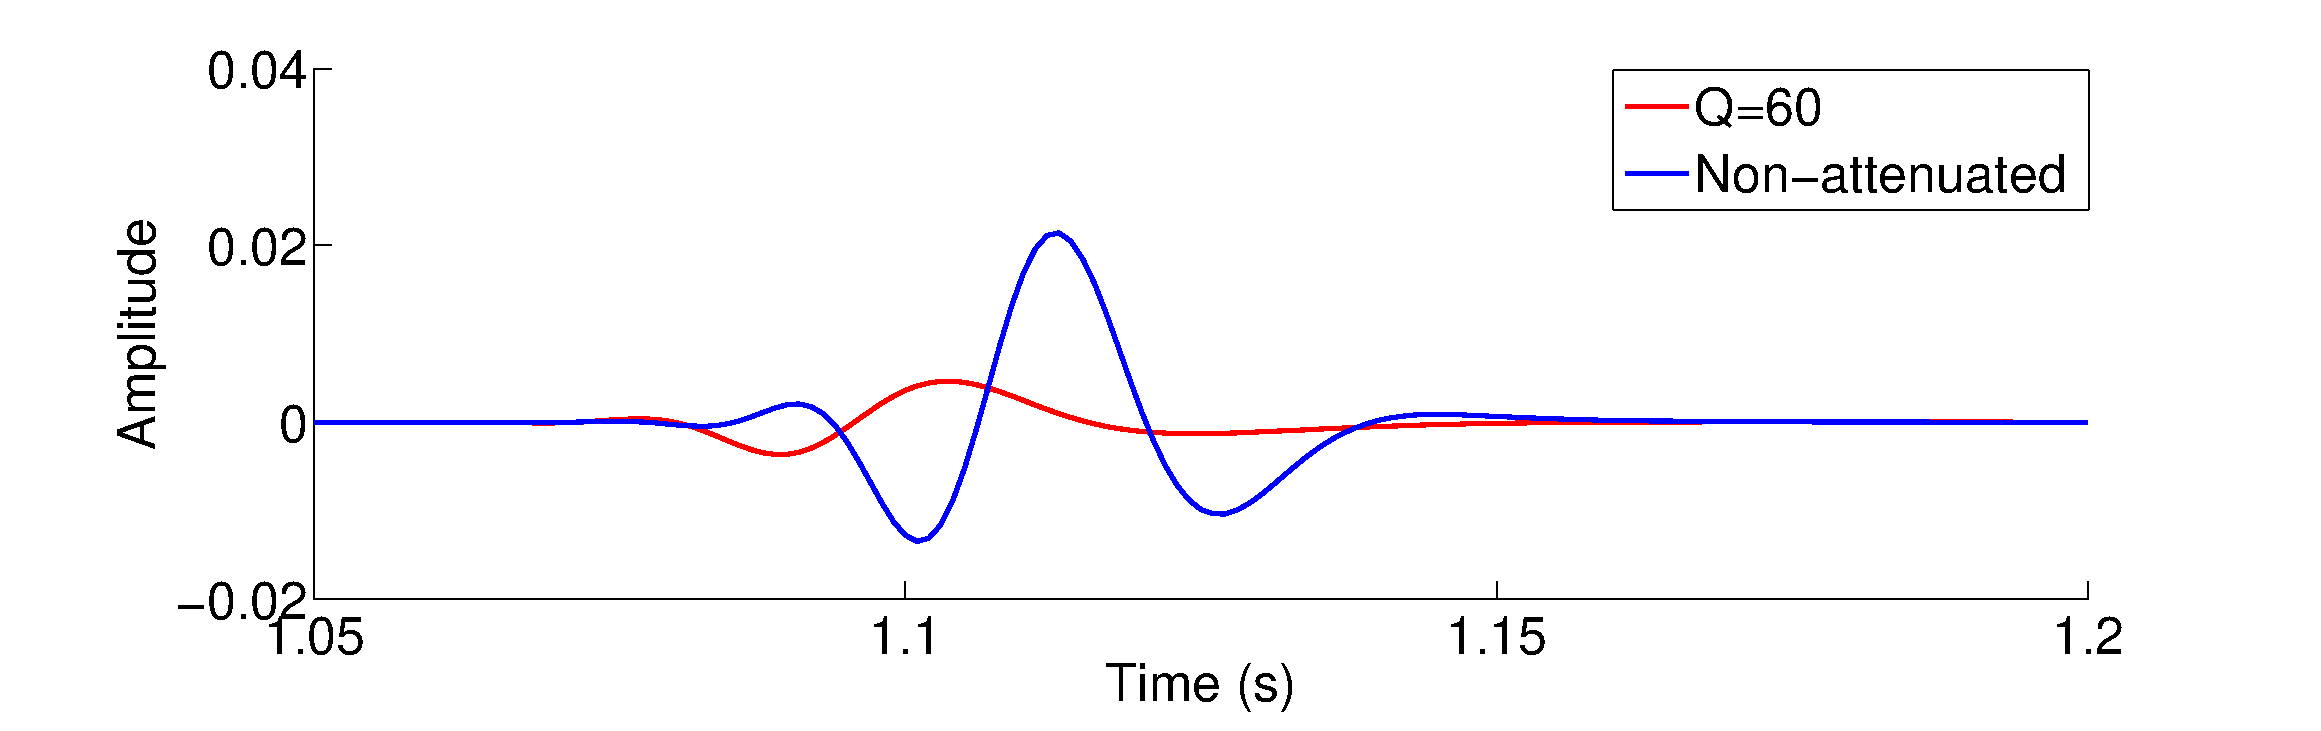
\includegraphics[width=0.9\linewidth]{figure/wavelet_ch1}}
		\subfigure[]{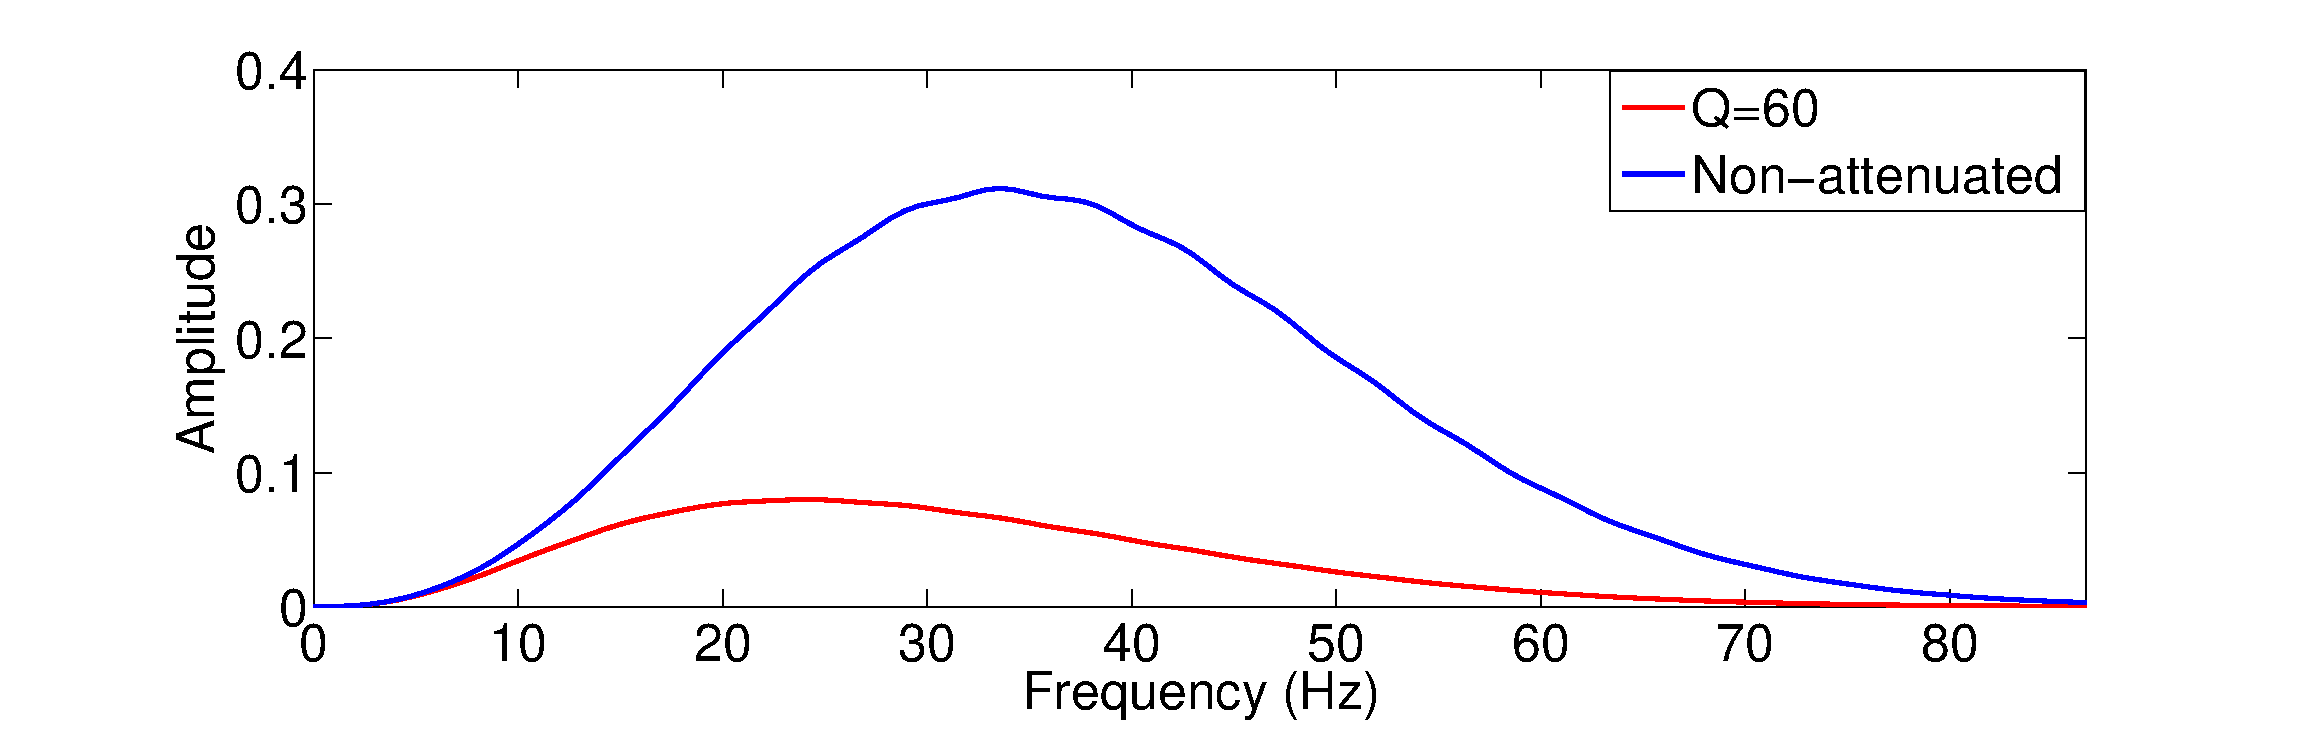
\includegraphics[width=0.9\linewidth]{figure/spectrum_ch1}}
        \fcaption{地震波在声介质和粘声介质($Q=60$)中传播的数值模拟实验:
	(a)地震波波形图;(b)对应的振幅谱。}{1D example to numerically illustrate the attenuation 
	impacts on the amplitudes spectra and phase of propagating wave: (a) the 
	non-attenuated waveform (blue curve) and the attenuated waveform (red curve); (b) the 
	corresponding amplitude spectral. }[展示地震衰减效应的一维数值实验]
        \label{fig:spectral}
\end{figure*}

在地震波偏移成像中,如果不补偿$Q$的效应,同样会影响地震成像的质量。地震衰减通过吸收地震波的
高频成分和改造地震波的相位来降低地震波成像的质量。图(\ref{fig:qrtm}c)展示了用准确$Q$补偿的
逆时偏移($Q$-RTM)成像结果。像被精确地成在了深度为800m的地方,并且像在强衰减区域下面有
均衡的能量。图(\ref{fig:qrtm}d)是没用$Q$补偿的RTM结果。由于频散的速度在成像中
没有得到校正,成像的位置要稍微浅于800m,并且在强衰减区域下方成像能量弱。在地震勘探过程,
不考虑$Q$的影响可能会导致地震解释不准确,甚至导致钻井错位。

\begin{figure*}[!htbp]
        \centering
		\subfigure[]{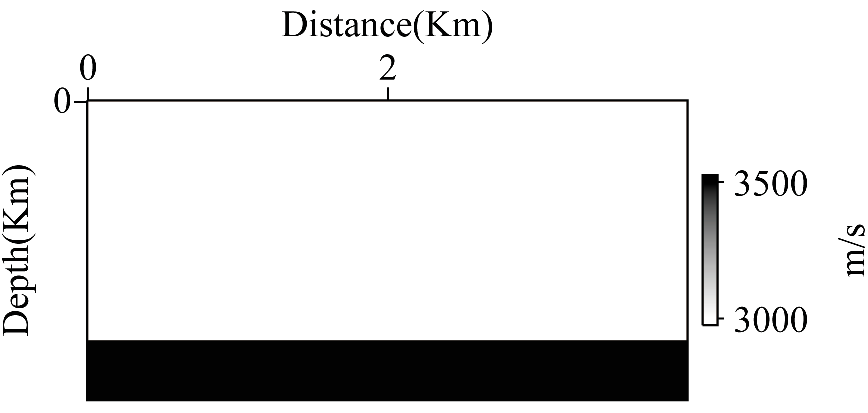
\includegraphics[width=0.495\linewidth]{figure/modelv_ch1}}
		\subfigure[]{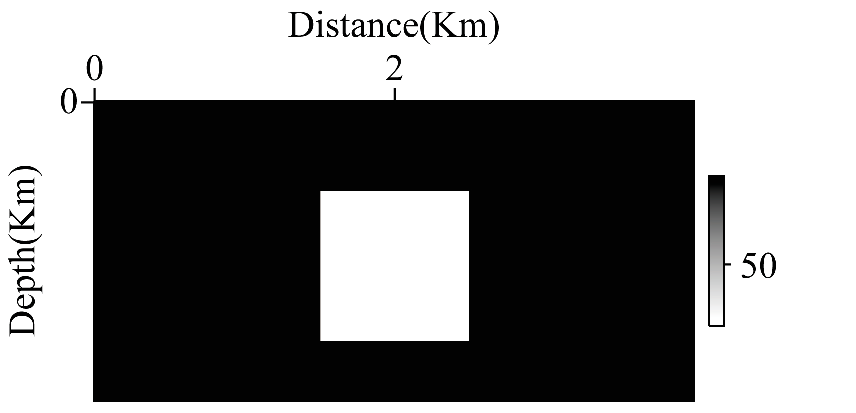
\includegraphics[width=0.495\linewidth]{figure/modelq_ch1}}
		\subfigure[]{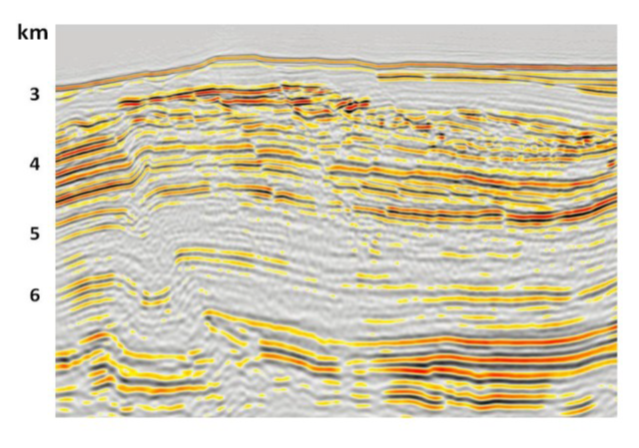
\includegraphics[width=0.495\linewidth]{figure/mig_q_ch1}}
		\subfigure[]{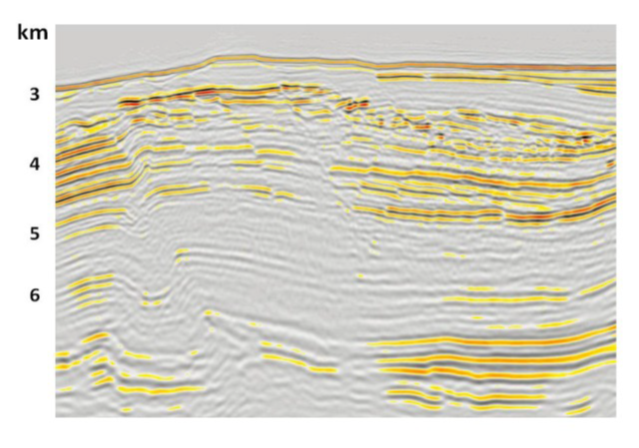
\includegraphics[width=0.495\linewidth]{figure/mig_no_ch1}}
		\fcaption{衰减对成像的影响实验:(a) 速度模型; (b)$Q$模型;(c)$Q$-RTM成像结果;
		(d)RTM成像结果}{ (a) The velocity model. (b) The $Q$ model.
		(c) The migrated image with a correct $Q$ compensation. (d) The migrated image without
		$Q$ compensation.}[衰减对成像的影响实验]
        \label{fig:qrtm}
\end{figure*}

在实际勘探中,汽云/包区的成像、储层识别和解释都面临巨大的挑战。汽云/包区通常包含极低的
$Q$值,这种强烈的衰减会吸收深部同相轴的能量,在储层的上方造成成像阴影区,严重影响地震
解释的准确性。可靠的$Q$模型不仅可以提高成像的质量,而且可以更好解释振幅随偏移距变化
(AVO)和各向异性这两种依赖于偏移距的效应。正确的AVO和各向异性
解释可以提高油气勘探的成功率。另外,$Q$模型可以作为一个表征岩石和流体属性的参数,
例如在稀疏井约束下,可以用$Q$模型来检测岩性的边界(\citeA{desgupta.clark:1998})。
衰减量级是一个直接刻画储层的油气物理参数,例如可以直接利用$Q$模型来确定储层含油/气
的饱和度(\citeA{winkler.nur:1982})。在油气开发过程中,衰减模型还可以用来指示储层裂缝的方位
(\citeA{maultzsch.chapman:2007}; \citeA{clark.benson:2009})以及监控流体的运移能力,
帮助优化注水过程(\citeA{macrides.kanasewich:1987})。
因此,在油气勘探开发过程中,定量地评估衰减效应,构建一个可靠的衰减($Q$)模型是非常重要的。
本文主要的工作就是通过反射全波形反演来定量估计地震本征衰减$Q$模型。

\vspace{1.2cm}
\section{国内外研究现状}
\vspace{0.4cm}

国内外学者对$Q$模型估计做了大量的研究工作,其中大部分工作都是在数据域完成。数据域的
反演方法可大致分为两类:基于高频近似的射线层析类和基于波动方程的波形反演类。

射线类方法中,\citeB{brzostowski.mcmechan:1992}首先用观测数据振幅与震源振幅比值的对数作为输入数据来
实现$Q$层析成像。但是除了吸收衰减外,影响振幅的因素还有很多如几何扩散、透射/反射损失、
散射损失等。为了区分衰减引起的振幅损失,\citeB{quan.harris:1997}将观测数据和计算数据间质心
频率的移动作为匹配准则,用射线层析方程来更新$Q$模型。\citeB{hu.liu:2011}用震源的振幅谱作为
拟合函数来处理地震数据频谱非对称性的影响,并用多指数盒状约束法来消除非地震本征衰减的影响。
质心频率移动类的方法相对于振幅匹配类方法对噪音不敏感,所以更适合于处理实际数据。
射线类方法计算效率高,处理简单横向变化的地质构造有很好的效果。但是在上覆介质复杂时,
地震波存在多路径,射线类方法由于不能处理多路径情况而造成误差。波动类层析方法可以
有效的解决多路径问题。

波形反演(FWI)是一种通过求解波动方程来恢复地下介质参数的反演迭代方法(\citeA{tarantola:1984})。
尽管FWI是一个高度非线性的反演问题(\citeA{mora:1987};\citeA{sirgue.pratt:2004}),由于需要
大量的正演计算,全局寻优的解法(\citeA{sen.stoffa:1991};\citeA{mosegaard.tarantola:1995})
所需的计算量仍是现在计算机所不能承受的。伴随状态法的引入(\citeA{lailly:1983};
\citeA{tarantola:1984};\citeA{pratt.worthington:1990}),使得梯度的计算变得非常高效,目前基于
梯度类的解法已趋于成熟。在勘探地震学中,各种应用实例证明粘声波形反演($Q$-FWI)对于提供高
分辨率的P波速度结构有非常重要的作用(\citeA{song:1995};\citeA{ravaut:2004} 
;\citeA{gao:2006}; \citeA{kamei:2012})。但是衰减的波形反演比速度的波形反演更具挑战性(
\citeA{song:1995};\citeA{liao.mcmechan:1996};\citeA{smithyman:2009};\citeA{hak.mulder:2011} 
;\citeA{malinowski:2011};\citeA{bai:2014};\citeA{kamei.pratt:2013})。

考虑衰减参数的波形反演第一次出现在\citeB{tarantola:1988}的时间域粘弹波形反演理论中。
随后,\citeB{song:1995}在频率域提出了一种粘声波形反演方法。在频率域实现波形反演比时间域
有如下优势,尤其是考虑衰减效应: 首先,衰减参数(例如$Q$值)和频散速度关系很容易用随频率
变化的复速度来表示,速度和衰减参数的梯度可以同时得到而不需要额外的计算量(\citeA{song:1995})。
另外,频率域反演方法可以自然的实现多尺度反演策略以降低波形反演的非线性(\citeA{bunks:1995};
\citeA{sirgue.pratt:2004})。从最低的频率成分开始反演,并逐渐增加高频成分,这样可以
逐渐恢复地下模型的高波数成分。

在波形反演中,速度和衰减参数$Q$有很强的耦合性(\citeA{song:1995};\citeA{kamei.pratt:2008};
\citeA{hak.mulder:2011})。\citeB{ribodetti:2000}以及\citeB{hak.mulder:2010}讨论了观测系统的
重要性,他们指出,完美的地下照明可以解决这种参数串扰问题。\citeB{innanen.weglein:2007}用逆散射
理论和一阶的频散反射系数来区分一维速度和衰减系数结构。\citeB{mulder.hak:2009}调查了
线性Born反演的零空间情况,并且指出,在计算梯度时如果不考虑速度频散关系,对于给定的地表反射数据,
地下许多速度/衰减对存在无解的情况。\citeB{hak.mulder:2011}指出,对于地表观测系统,考虑了频散关系
的非线性波形反演可以较精确地反演简单二维合成模型的速度和衰减系数。
然而,在早些阶段的反演中,串扰线性还是很明显,并且需要非常多(在他们的实验中大于10000次)的迭代
次数来消除假象,因此该反演问题还是非常病态的。

在$Q$-FWI中,各种各样的预条件方法被用来减弱其反演的病态性。\citeB{liao.mcmechan:1996}用合成数据
实验显示要获得好的衰减模型,必须要对模型参数进行一定的范围约束。\citeB{hak.mulder:2011}指出
基于两种参数特征值的大小来惩罚梯度中衰减成分可以加速$Q$-FWI的收敛。\citeB{malinowski:2011}
在波兰的盆地中成功的反演出了与可用的岩性信息一致的衰减模型。他们指出对地震数据时间方向强阻尼衰减
和梯度大尺度平滑约束是反演$Q$参数的关键。

对于$Q$反演的另一类做法是顺序反演,先获取比较准确的速度模型然后再反演$Q$模型。如果我们认为
前期的振幅变化主要是由于速度结构引起的,后续再反演$Q$时可以降低反演的串扰。初始的速度估计是通过
固定衰减模型反演的(\citeA{pratt:2004};\citeA{kamei.pratt:2008};\citeA{rao.wang:2008};
\citeA{smithyman:2009})。\citeB{pratt:2004}用顺序反演法来处理含碳水化合物的强衰减跨井数据。
对于$Q$模型的反演,他们也用了较大的平滑约束,其反演结果与超声波形分析结果有很好的一致性。
\citeB{watanabe:2004}在超声频段用实验室数据同样很好实现了顺序反演方法。\citeB{smithyman:2009}
用顺序反演法来识别近地表目标。\citeB{watanabe:2004}以及\citeB{kamei.pratt:2008}用合成跨井数据
比对了同时反演和顺序反演的结果,在没有正则化项的情况下,顺序反演会得到更好的结果。
\citeB{kamei.pratt:2008}认为地震数据中大部分振幅变化是由速度变化引起的。
\citeB{kamei.pratt:2013}系统地调查了不同梯度预条件对$Q$反演的影响。

地震数据的走时信息主要受速度参数影响,地震衰减通过频散关系照样影响走时,但衰减主要影响
地震的振幅信息。相较于走时信息,地震振幅很容易受噪音、震源检波器的耦合、震源的辐射模式以及
弹性(非声学)效应。为了保证振幅信息的准确性,需要非常细心的前处理工作(\citeA{pratt:2004};
\citeA{malinowski:2011})。\citeB{dutta.schuster:2016}通过将峰值频率移动引入到$Q$-FWI中
来降低数据对前处理的依赖,从目标函数出发降低了$Q$-FWI的非线性程度。

FWI需要低频全方位大孔徑地震数据,但是这种高质量的数据采集往往需要高昂的采集费用。
通过不同观测孔径的观测系统照明分析可知,当缺少大孔径的折射波数据时,深部模型往往只被
反射波照明,目前海上勘探最为普遍的拖缆数据(缆长一般5至6公里)正是这种情况。
因此,利用反射波进行中深部的速度建模已成为地震成像的共识。
但是,当利用反射数据进行常规的FWI时,其梯度中高频成分占主导,反射波的偏移响应与利用反射波反演
背景模型的核函数相比,数值上往往高一个数量级。在常规的反射FWI中,往往只会得到一个
高波数的成像结果,不易于更新背景模型(\citeA{wu.alkhalifah:2014};\citeA{alkhalifah:2015};
\citeA{chi:2015};\citeA{alkhalifah.wu:2016})。
因此,为增强对模型低频成分的更新,学者们提出了波场分解的方法(\citeA{Liu:2011};\citeA{wang:2013};
\citeA{tang:2013}),目的是增强层析分量的贡献进而得到有效的长波长分量更新。

为了解决反射波数据应用FWI时的上述问题,\citeB{xu:2012a}在全波形反演的框架下,提出了反射波波形反演
方法(RWI)。RWI的思想在于:利用反射地震数据反演模型参数时,首先更新背景速度而非高波数的速度扰动,
这样的反演策略更加有利于反演收敛,这是对常规FWI思路的很好补充。RWI将速度模型分解为背景模型和扰动模型
两部分,并分别给出了地震波场对于背景模型和扰动模型的Frechet导数。

但是,为了使RWI能够在实际地震资料反演中更好的恢复中深层背景速度,必须进行数据匹配和真振幅偏移
(反射系数估计)。\citeB{ma.hale:2013}利用DIW算法(Dynamic image warping)提取反射波的走时时差,
实现中深层背景速度建模,提高反演的稳定性。\citeB{alkhalifah:2016}用反射角滤波的全模型反演方法
来解决数据匹配问题。基于相关的反射波波形反演方法(\citeA{chi:2015}),在一定程度上也避免了
数据匹配的周期跳跃问题。即使在观测数据中缺乏有效低频信息、背景模型相对较差时,RWI也可以较好的
恢复模型中深部的低波数成分。在反射系数估计方面,最小二乘偏移(\citeA{dai.schuster:2013};
\citeA{zhang:2014})是目前比较有效的方法。但是,最小二乘偏移要求背景模型要足够准确
(\citeA{luo.hale:2014}),否则当背景速度不准确时,其反演的高波数模型扰动也不正确,而这又与
RWI反演背景速度的目标相矛盾。因此,在反射波波形反演中,如何以及何时引入最小二乘偏移将显得非常重要。

\citeB{shen.biondi:2018}在成像域建立起了模型扰动与像扰动的关系,通过$Q$偏移分析获取中深层的背景$Q$模型。
在数据域,目前还没人探讨用地表地震数据恢复中深层背景$Q$模型。本文将研究如何把RWI引入到背景$Q$反演中。

\vspace{0.9cm}
\section{本文研究内容}
\vspace{0.5cm}

地震衰减参数$Q$对地震波振幅的影响类似于速度对走时信息的影响,是一种沿地震波路径累积叠加效应,
并且主要与模型的低波数背景成分有关。在实际应用中,相对准确的低波数背景$Q$模型即可补偿成像中
能量的损失,同时也能帮助储层、岩性解释。本文结合地震衰减的具体特点,将RWI引入到
背景$Q$反演中,以实现中深层背景衰减模型的反演。具体研究内容包括:

在第二章中,首先简单回顾了地震衰减的基本理论,重述表征地震衰减的物理参数(品质因子和吸收系数);
其次系统地总结了描述地震衰减的不同力学模型,并重点讲述了勘探地震中常用的两类模型(标准线性固体模型
和常$Q$模型);然后推导了描述这两类衰减模型对应粘声波方程,并比较了这两种方程模拟的结果;最后较为
完整的总结了$Q$补偿的逆时偏移($Q$-RTM)所遇到的问题及其解决办法,并比较了上述两类方程在$Q$偏移
成像中的应用。

在第三章中,在顺序反演的背景下,提出了粘声反射全波形反演($Q$-RWI)方法。假定速度准确,将速度分解为
背景和扰动两部分,基于标准线性固体模型粘声方程通过Born实现上下行波的分离。在RWI的框架下,用数据残差的
目标函数更新中深层背景$Q$模型。

在第四章中,通过引入峰值频率移动的目标泛函来降低$Q$-RWI对高频扰动速度的依赖性。

最后,总结论文的主要结论和创新点,讨论不足之处以及未来的研究方向。

















